% FluxV v5a/v5b joint stage summary (fail-closed)
\begin{figure}[t]
  \centering
  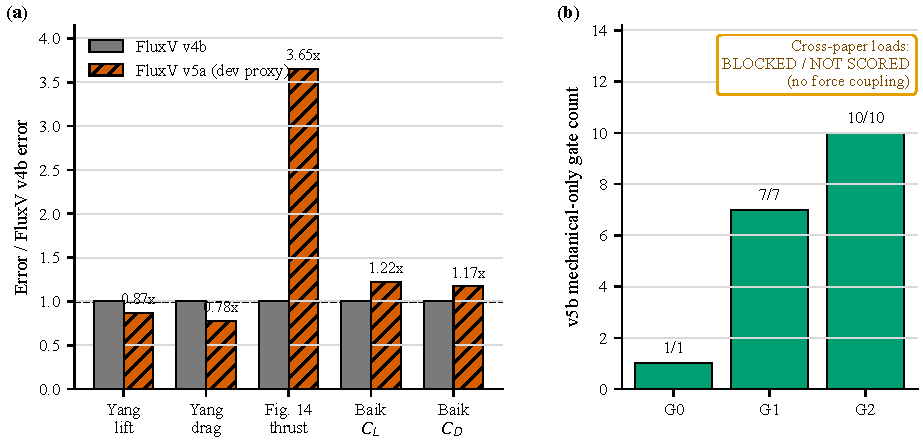
\includegraphics[width=0.95\textwidth]{fluxv_v5_joint_stage_summary.pdf}
  \caption{FluxV v5 staged evidence. (a) Frozen development-only v5a error normalized by v4b error; lower is better. Metrics are Yang cycle-mean MAE, Figure 14 all-14 CT RMSE, and Baik 1-Hz-filtered waveform macro RMSE. (b) v5b G0--G2 topology/conservation gate counts. The v5b shared-wake smoke has no force coupling, so cross-paper load accuracy is blocked and not scored. Sample scopes are Yang: 6 conditions; Figure 14: 14 points; Baik: 4 waveforms with 400 unique phase samples each.}
  \label{fig:fluxv-v5-joint-stage}
\end{figure}
